\chapter{データ実験の詳細}
\label{chap:data}
\section{使用したモデルの詳細}
第3章で述べたとおり使用した対戦データは弱いAIを先番とし,強いAIを後手としている.
AIの強さは一手ごとの探索を行う時間(time),付録Cで述べる$C_{puct}$,ニューラルネットワークの訓練段階におけるエポック数の値によって調整した.
timeと$C_{puct}$,エポック数はいずれも値が大きい程モデルは強くなると考えられる.(エポック数については付録\ref{chap:baseline}を参照)
対戦データ生成時のパラメータは表\ref{table:param-battle}の幅からゲームごとにランダムな値を採用した.
これはパラメータの値を変化させることでゲームデータに多様性を持たせるためである.
\begin{table}[H]
	\caption{対戦データのパラメータ}
	\label{table:param-battle}
	\centering
	\scalebox{0.98}[0.98]{
		\begin{tabular}{c|c|c}
			モデル&強&弱\\ \hline
			time    & 3-5 & 0-2 \\ 
			$C_{puct}$ & 0.8-1   & 0-0.5 \\
			エポック数 & 200 & 1 \\

		\end{tabular}
	}
	\label{table:battle}
\end{table}

\section{対戦結果の詳細}
2000ゲームのうち1983ゲームは強いAI(後番)の勝利となった.
また,ゲームごとの手数は75\%のゲームが36手以内で終了している.
そのため,データ実験ではゲームの中盤と言える13$\sim$24手目のデータを使用した.
図\ref{fig:stepCum}にゲームの終了手数の累計グラフを示す.
\begin{figure}[htbp]
	\centering
	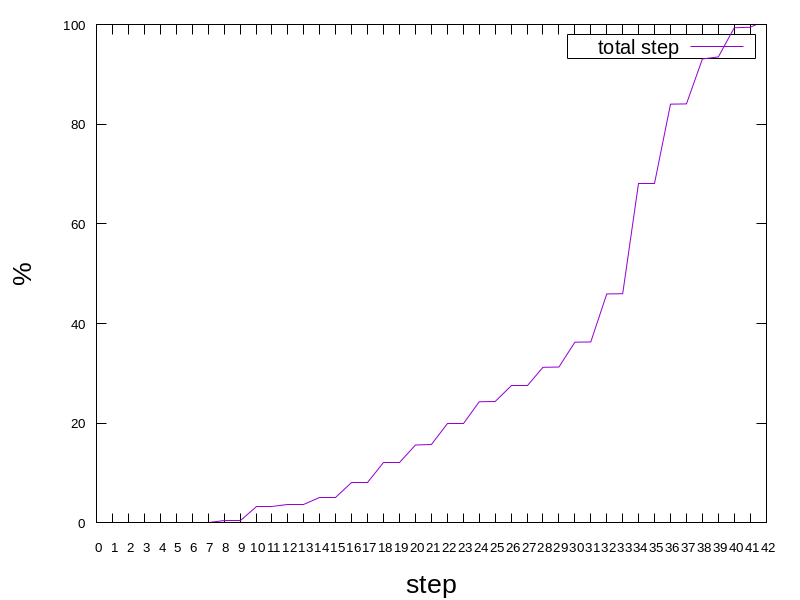
\includegraphics[width=\linewidth]{./figure/stepCum.png}
	\caption{終了手数の分布}
	\label{fig:stepCum}
\end{figure}




\section{データ実験に使用したモデルの詳細}
第4章に記載した表\ref{table:result-online}の結果を求める際に用いたモデルのパラメータを表\ref{table:param-data}に示す.
\begin{table}[H]
	\caption{データ実験:使用モデルのパラメータ}
	\centering
	\scalebox{0.98}[0.98]{
		\begin{tabular}{c|c}
			パラメータ名 & 値 \\ \hline
			time    & 対戦時の後番のモデルと同じ \\ 
			$C_{puct}$    & 対戦時の後番のモデルと同じ \\
			エポック数 & 200 \\
			$k$ (提案手法のみ)     & 4 \\
			$l$ (提案手法のみ)     & 2 \\
		\end{tabular}
	}
	\label{table:param-data}
\end{table}

表\ref{table:param-data}の通り,対戦データが生成された際のモデルのパラメータを使用している.
そのため本手法はモデルの構造とパラメータの値へのアクセスが可能な場合を想定したホワイトボックス的アプローチの実験であると言える.
モデルのtime, $C_{puct}$の値を固定して同様の手法を適用した場合の実験結果を\ref{sec:gray}で示す.
\section{末尾のグループ化}
提案手法は予想図とその予想図に至る軌跡(両方を合わせて進行図と記載)を抽出する.
図\ref{fig:regroup}は軌跡を末尾の3手で2つのグループに再編する様子を表している.(ここでは軌跡は行動$a$の連続として表している)
\begin{figure}[htbp]
	\centering
	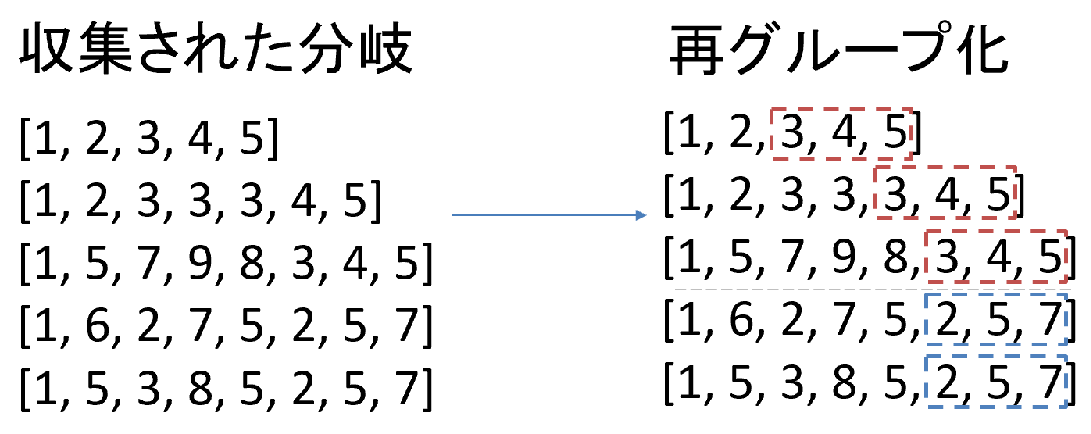
\includegraphics[width=\linewidth]{./figure/regroup.pdf}
	\caption{再グループ化}
	\label{fig:regroup}
\end{figure}
取り出された軌跡を末尾の3手の選択でさらにグループ化した結果,元の軌跡の数と再グループ化された軌跡の数の平均は
表\ref{table:tail}のようになった.
結果として,取り出された軌跡のうち,平均約2$\sim$3つの軌跡において末尾の3手が共通する傾向にあることがわかった.
\begin{table}[H]
	\caption{再グループ化した際の軌跡の数}
    \scriptsize
    \label{table:tail}
	\centering
	\scalebox{0.98}[0.98]{
		\begin{tabular}{c|c|c||c}
			手数(盤面数, 補間の有無)&  再グループ化前の軌跡数(平均)&  再グループ化後の軌跡数(平均)\\ \hline
			19-24(9862, 無)    & 7.01 & 3.00  \\
			19-24(9862, 有)    & 13.62 & 4.43  \\
			13-24(21022, 無)   &  6.95& 3.08  \\
			13-24(21022, 有)   & 12.93 & 4.51 \\
		    0-40(61021,無)& 5.23 & 2.23\\
		    0-40(61021,有)& 10.82 & 3.78\\
		\end{tabular}
	}

	
\end{table}
また,各軌跡の長さの平均は\ref{fig:length}のようになった.
尚,正確には1つの盤面,行動(最も探索回数が大きい行動)の組に対して取り出される軌跡の平均を更に平均した値を示している.
\begin{table}[H]
	\caption{軌跡の長さの平均}
    \scriptsize
    \label{fig:length}
	\centering
	\scalebox{0.98}[0.98]{
		\begin{tabular}{c|c}
			手数(盤面数, 補間の有無)&  軌跡の長さ(平均)\\ \hline
		    0-40(61021,無)& 10.89\\
		    0-40(61021,有)& 15.31\\
		\end{tabular}
	}	
\end{table}

\section{グレーボックス的手法}
\label{sec:gray}
モデルのパラメータを固定し,再び第4章のデータ実験を行った.パラメータの値を固定しているため,本実験はモデルの具体的なパラメータの値へのアクセスが不可能な場合にも適用可能な
グレーボックス的手法であると言える.
固定されたパラメータを表\ref{table:param-data-extra}に示す.
\begin{table}[H]
	\caption{データ実験(追加):使用モデルのパラメータ}
	\centering
	\scalebox{0.98}[0.98]{
		\begin{tabular}{c|c}
			パラメータ名 & 値 \\ \hline
			time    & 5 \\ 
			$C_{puct}$    & 1 \\
			エポック数 & 200 \\
			$k$ (提案手法のみ)     & 4 \\
			$l$ (提案手法のみ)     & 2 \\
		\end{tabular}
	}
	\label{table:param-data-extra}
\end{table}

実験の結果は表\ref{table:result-offline}のようになった.第4章に記載したホワイトボックス的手法と同様に提案手法はgroup prediction rateにおいて比較手法より高い値を示した.
\begin{table}[H]
	\caption{実験結果:データ実験}
	\centering
	\scalebox{0.98}[0.98]{
		\begin{tabular}{c|c|c|c|c}
			\multicolumn{1}{c}{} & \multicolumn{2}{|c|}{group prediction rate} 
			& \multicolumn{2}{c|}{stone prediction rate}\\ \hline \hline
			手数(盤面数, 補間の有無)  & 比較手法  & 提案手法 & 比較手法 & 提案手法  \\ \hline
			19-24(9862, 無) & 0.44& \bf{0.60} & \bf{0.63} & 0.61  \\
			19-24(9862, 有)  & 0.44   & \bf{0.63}& \bf{0.63} & 0.61   \\
			13-24(21022, 無)   & 0.37  & \bf{0.53}& \bf{0.56} & 0.55  \\
			13-24(21022, 有)   & 0.37 & \bf{0.55}& \bf{0.56} & 0.55   \\
		\end{tabular}
	}
	\label{table:result-offline}
\end{table}
